\chapter{数值实验}
\label{cha:numerical}
本章中主要对两个数据集来进行实验。一个取样于一个单位球面($S^2$),包含$1002$个点,另一个取样于一个牛形的曲面($Cow$),包含$2602$个点。本节中首先比较不同sampling rate下前述算法重构距离矩阵的相对误差,即
\begin{equation*}
    \text{Error} = \frac{\|\mathbf{X}-\mathbf{M}\|_F}{\|\mathbf{M}\|_F}
\end{equation*}
其中,由于数据是从点集中随机取样,故表格中用5次实验的误差的均值来进行比较。同时算法中的一些需要预先确定的参数,在没有特殊说明的情况下,参见前面各算法表述中   \textbf{Require}。

本节的实验主要分为三个部分,第一部分首先确认两个数据集所要带入OPTSPACE算法中的秩的大小。第二部分展示SMACOF, 和基于SVT还有OPTSPACE和经典多维尺度变换的算法,在处理不同sampling rate下两个数据集的结果。并对于数值实验的结果进行分析总结。最后一部分,我们分析比较各算法在两个数据集上的表现与效果,并分析产生差异的原因。


首先,先来判断两个数据集的秩。分别对两个数据集在sampling rate比较大的情况下分别用不同的秩带入算法,通过比较Error的情况来确定所要带入算法中的秩的大小。为此,本文中先针对sampling rate分别为$30\%, 50\%$和$70\%$的情况,将$rank = 1, 2, 3, 4, 5$分别带入参数为$tau = 10^{-3}$的OPTSPACE算法,然后选取使Error相对较小的秩中最小的一个。
\begin{table}[!htbp]
\centering
\begin{tabular}{|c|ccccc|}
\hline
\diagbox{rate}{Error}{rank}&1 &2 &3 &4 &5\\
\hline
\text{30\%}&0.3375 &0.2278 &0.1982 &1.094E-4 &1.095E-5 \\
\hline
\text{50\%}&0.3372 &0.2773 &0.1977 &9.758E-5 &9.887E-5\\
\hline
\text{70\%}&0.3370 &0.2770 &0.1974 &6.300E-5 &6.351E-5\\
\hline
\end{tabular}
\caption{$S^2$数据集sampling rate为30\%,50\%和70\%情况下秩为1\~{}5分别带入OPTSPACE算法作为参数的Error}
\label{tab: sphere_rank}
\end{table}

\begin{table}[!htbp]
\centering
\begin{tabular}{|c|ccccc|}
\hline
\diagbox{rate}{Error}{rank}&1 &2 &3 &4 &5\\
\hline
\text{30\%}&0.4586 &0.1411 &0.0686 &0.0686 &0.0686 \\
\hline
\text{50\%}&0.4583 &0.1411 &0.0685 &0.0428 &0.0428\\
\hline
\text{70\%}&0.4584 &0.1410 &0.0685 &0.0412 &0.0159\\
\hline
\end{tabular}
\caption{$Cow$数据集sampling rate为30\%,50\%和70\%情况下秩为1\~{}5分别带入OPTSPACE算法作为参数的Error}
\label{tab: cow_rank}
\end{table}

由表\ref{tab: sphere_rank}和表\ref{tab: cow_rank}可见,对于$S^2$中各个sampling rate,Error都是在秩为$4$的带入算法的时候最小。对于$Cow$数据集中当sampling rate为$70\%$时,当秩为$5$的时候Error才达到最小。故$S^2$数据集应带入$rank = 4$,$Cow$数据集中应带入$rank = 5$。同时从表\ref{tab: cow_rank}中可以看见当sampling rate为$30\%$时,从$rank = 3$开始,Error已经不再发生变化,并观察到在$30\%, 50\%, 70\%$这样较大的sampling rate下,$Cow$数据集中的Error仍然很大。由此可以预估$Cow$数据集可能存在条件数比较大的情况,并进而影响了OPTSPACE算法在该数据集上的效果。在后面的实验中也验证了我们这一猜测。



%\begin{figure}
%\centering 
%\includegraphics[totalheight=4.8in]{SpherePlot.png} 
%\caption{不同sampling rate下$S^2$三种算法恢复结果图} 
%\label{fig:sphere} 
%\end{figure}
\begin{figure}[h]
	\centering
	\includegraphics[width=1.0\textwidth]{figure/SpherePlot.png}
	\caption{不同sampling rate下三种算法恢复$S^2$数据集结果图}
 	\label{fig:sphere}
\end{figure}

\begin{table}[!htbp]
\caption{不同Sampling Rate下不同算法重构的$S^2$距离矩阵的误差}
\label{tab: sphere}
\centering
\begin{tabular}{|c|ccccc|}
\hline
\diagbox{Algorithm}{Error}{Sampling rate}&$2\%$ &$3\%$ &$5\%$ &$10\%$ &$20\%$\\
\hline
\text{SMACOF}&0.0200 &2.070E-4 &1.162E-4 &4.7375E-4 &2.9069E-5 \\
\hline
\text{SVT+CMDS}&0.1889 &1.731E-4 &1.753E-4 &1.450E-4 &1.289E-4\\
\hline
\text{OPTSPACE+CMDS}&0093 &4.4196E-4 &1.7065E-4 &1.3347E-5 &1.2121E-4\\
\hline
\end{tabular}
\end{table}
接下来,在图\ref{fig:sphere}中展示了SMACOF和先用SVT, OPTSPACE算法恢复距离矩阵之后再用经典多维尺度变换算法恢复不同sampling rate下$S^2$数据集的结果。表\ref{tab: sphere}中展示了三种算法,在不同sampling rate下的Error。可以看到整体来说三种方法的效果都是挺理想的,除了在sampling rate为$2\%$时SMACOF和SVT两种方法的误差较大,在图中明显可以看出SMACOF恢复的结果在球面在一些地方有突起的异常值,而SVT算法的结果更是无法观察出光滑的球面。但除此之外,三种算法在各个sampling rate下都达到了$10^{-4}$数量级的误差精度。
\begin{figure}[h]
	\centering
	\includegraphics[width=1.0\textwidth]{figure/CowPlot.png}
	\caption{不同sampling rate下四种算法恢复$Cow$数据集结果图}
 	\label{fig:cow}
\end{figure}
%\begin{figure}
%\centering 
%\includegraphics[totalheight=4.8in]{CowPlot.png} 
%\caption{不同sampling rate下$S^2$四种算法恢复结果图} 
%\label{fig:cow} 
%\end{figure}

\begin{table}[!htbp]
\caption{不同Sampling Rate下不同算法重构的$Cow$距离矩阵的误差}
\label{tab:COW}
\centering
\begin{tabular}{|c|ccccc|}
\hline
\diagbox{Algorithm}{Error}{Sampling rate}&$2\%$ &$3\%$ &$5\%$ &$10\%$ &$20\%$\\
\hline
\text{SMACOF} &0.0065 &0.0054 &1.200E-4 &7.277E-5 &4.678E-5 \\
\hline
\text{SVT + CMDS} &0.0016 &7.029E-4 &3.187E-4 &2.713E-4 &2.449E-4\\
\hline
\text{OPTSPACE + CMDS}&0.1449 &0.2882 &0.0695 &0.0414 &0.0412\\
\hline
\text{IncOPTSPACE + CMDS}&0.0021 &0.0021 &1.521E-4 &0.0041 &0.0039\\
\hline
\end{tabular}
\end{table}

在图\ref{fig:cow}中展示了SMACOF,SVT + CMDS,OPTSPACE + CMDS,Incremental OPTCPACE + CMDS, 在sampling rate分别为$2\%, 3\%, 5\%, 10\%$下恢复$Cow$数据集的结果。同时表\ref{tab:COW}中展示了上述四个算法在不同sampling rate下的Error。不难发现OPTSPACE + CMDS的方法效果的确很差,进一步观察可以发现OPTSPACE在sampling rate为$2\%$和$3\%$时,恢复的坐标结果集中在一条直线附近。而在sampling rate为$5\%$和$10\%$时,虽然能看出大致牛的形状。但从图\ref{fig:cow_opt_20}中可以看到,当将sampling rate为$20\%$下用OPTSPACE + CMDS算法恢复出来的结果从侧面观察时,坐标集中在一个二维平面上,并不能表现出三维空间中立体的牛的形状。

\begin{figure}[h]
	\centering
	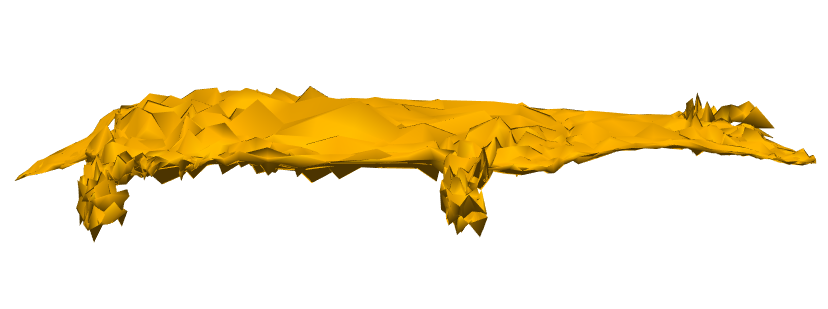
\includegraphics[width=1.0\textwidth]{figure/Cow_opt_20.png}
	\caption{sampling rate = $20\%$时OPTSPACE + CMDS恢复坐标结果的侧面图}
 	\label{fig:cow_opt_20}
\end{figure}

造成这样的原因可能就是前面所说的,前两个奇异值相较于之后的奇异值来说太大。事实上完整的$Cow$数据集的奇异值分别为$2.243\times10^3, 1.676\times10^3, 0.349\times10^3, 0.130\times10^3, 0.088\times10^3$,可以明显的发现前两个奇异值与后面三个之间的差值。同时,在前两个奇异值之间我们也能看到很明显的区别。这就验证了我们之前所说的OPTSPACE算法在矩阵条件数较大的时候效果不佳。而Incremental \\
OPTSPACE + CMDS方法相对于OPTSPACE算法来说有很大的改进。在此说明一下在应用Incremental OPTSPACE算法的过程中会发现即使每一次只计算最大的奇异值仍然不能保证有较好的效果,因此想到通过改变trimming过程和步长初值$tau$来进一步改善Incremental OPTSPACE。表\ref{tab:COW}中展示的结果为sampling rate分别为$2\%, 3\%, 5\%, 10\%, 20\%$时,trimming过程为将degree大于$1, 1, 0.8, 0.7, 0.7$倍的矩阵degree均值的行列置为零,初始步长$tau$设为$10^{-2}, 10^{-2}, 10^{-2}, 10^{-1}, 10^{-1}$时的结果。这样改变trimming过程的想法是希望在初次进行奇异值分解的时候能削弱degree较大的行与列,即较大的奇异值所产生的影响。在这样的操作之后,Incremental OPTSPACE算法的效果在原有基础上有了进一步的改善。


\begin{table}[!htbp]
\caption{SMACOF\ SVT+CMDS\ OPTSPACE+CMDS三种算法在恢复$S^2$数据集收敛或达到迭代次数上限所用时间}
\label{tab:SPHERE_TIME}
\centering
\begin{tabular}{|c|ccccc|}
\hline
\diagbox{Algorithm}{Time(s)}{Sampling rate}&$2\%$ &$3\%$ &$5\%$ &$10\%$ &$20\%$\\
\hline
\text{SMACOF} &394.3920 &120.7250 &68.6260 &90.1370 &40.6080 \\
\hline
\text{SVT + CMDS} &4246.1 &112.7820 &43.1310 &23.3750 &32.0340\\
\hline
\text{OPTSPACE + CMDS}&327.7620 &277.9470 &84.3620 &29.0830 &12.4380\\
\hline
\end{tabular}
\end{table}

\begin{table}[!htbp]
\caption{SMACOF\ SVT+CMDS\ OPTSPACE+CMDS三种算法在恢复$Cow$数据集收敛或达到迭代次数上限所用时间}
\label{tab:COW_TIME}
\centering
\begin{tabular}{|c|ccccc|}
\hline
\diagbox{Algorithm}{Time($10^3$s)}{Sampling rate}&$2\%$ &$3\%$ &$5\%$ &$10\%$ &$20\%$\\
\hline
\text{SMACOF} &4.7887 &4.7026 &2.1574 &2.0956 &2.5769 \\
\hline
\text{SVT + CMDS} &2.8380 &2.6550 &1.9729 &1.6608 &1.3542\\
\hline
\text{OPTSPACE + CMDS}&1.0910 &2.6439 &1.0924 &1.2613 &1.2763\\
\hline
\end{tabular}
\end{table}


\begin{figure}[h]
	\centering
	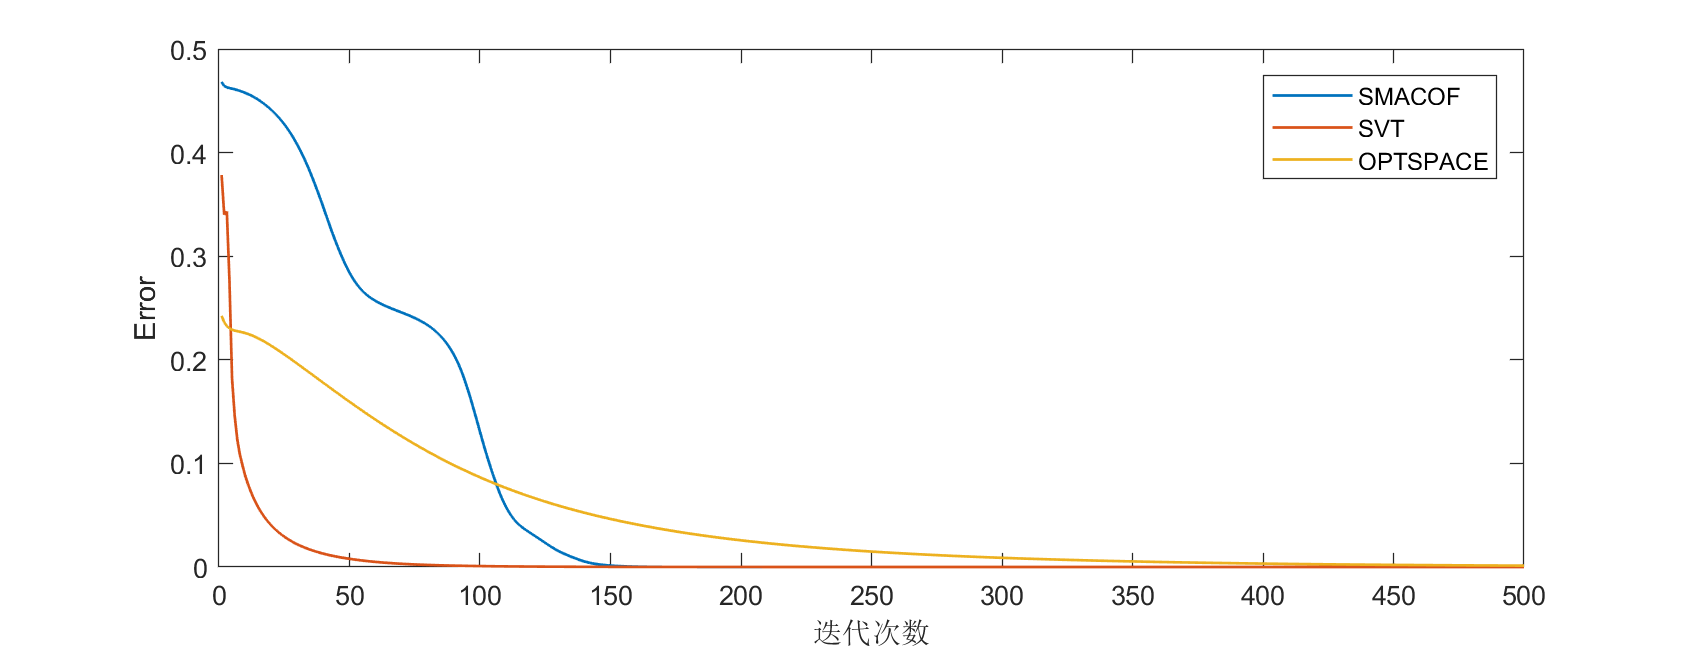
\includegraphics[width=1.0\textwidth]{figure/SphereError.png}
	\caption{sampling rate = $20\%$时三种算法恢复$S^2$数据集时Error随迭代次数变化曲线}
 	\label{fig:sphere_error}
\end{figure}


\begin{figure}[h]
	\centering
	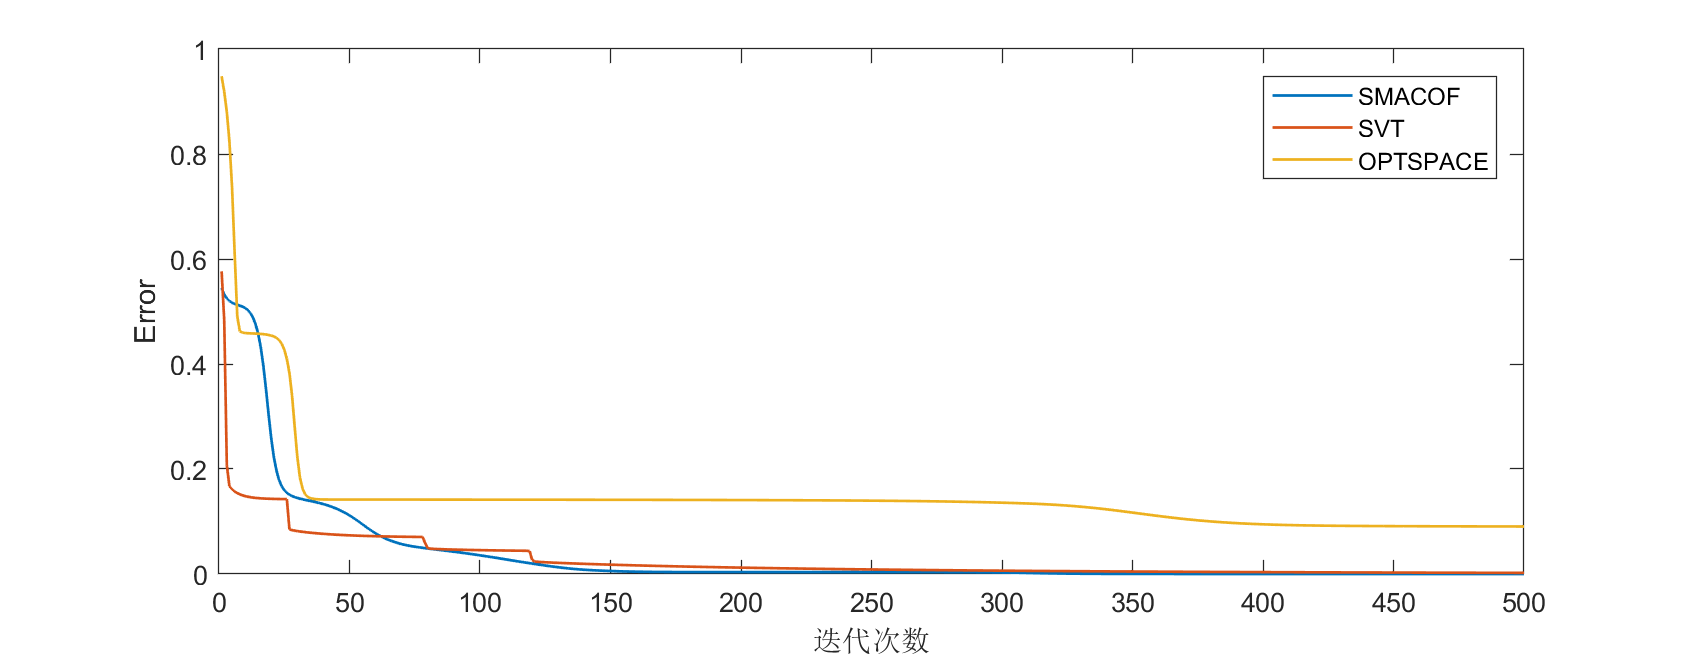
\includegraphics[width=1.0\textwidth]{figure/CowError.png}
	\caption{sampling rate = $20\%$时三种算法恢复$Cow$数据集时Error随迭代次数变化曲线}
 	\label{fig:cow_error}
\end{figure}

为进一步分析比较SMACOF, SVT + CMDS和OPTSPACE + CMDS三种算法,在表\ref{tab:SPHERE_TIME}和表\ref{tab:COW_TIME}中列出了三种算法收敛或达到最大迭代次数(1000次)所用的时间。在图\ref{fig:sphere_error}和图\ref{fig:cow_error}中展现了三种算法在两个数据集sampling rate为20的情况下,500次迭代内,Error随迭代次数的变化曲线。由于Incremental OPTSPACE + CMDS相对于其余三种算法来说多了一层对秩的循环,故不在此一起讨论。

首先,由表\ref{tab:SPHERE_TIME}和图\ref{fig:sphere_error}可以看出对于对于sampling rate为$20\%$下的$S^2$数据集,SMACOF和SVT + CMDS两个算法收敛速度很快,在前150次迭代内就可以将Error控制在一个很小的范围内。而OPTSPACE + CMDS相对于SMACOF + CMDS和SVT + CMDS而言,收敛曲线相对平缓,但却在整体用时上有明显的优势。由此可见OPTSPACE + CMDS在单次迭代过程中的运算速度很快。针对于整体其他sampling rate下的情况可以看出,SVT + CMDS算法可以在相对较短的时间和迭代次数内达到较为理想的精确度。同时如果更进一步的,在实验中使用稀疏矩阵的方式存储矩阵序列中的$\{\mathbf{Y}^k\}$,可以进一步提升运算速度。在$Cow$数据集中我们也可以得到类似的结论。由图\ref{fig:cow_error}中可以看出,和图\ref{fig:sphere_error}中一样,SMACOF + CMDS和SVT + CMDS也在200次的迭代内,误差很快就收敛到了相对较小的值,而OPTSPACE + CMDS在500次迭代之后仍保持着接近0.1的误差。这与我们之前直接对于恢复结果进行观察所得到的结论一致。在图\ref{fig:cow_error}中也可以看出OPTSPACE + CMDS算法在恢复$Cow$数据集中所存在的问题。由前面的算法描述可知,SVT + CMDS和OPTPACE + CMDS两种算法本质上都是基于奇异值分解。在SVT + CMDS算法的Error变化曲线中,我们可以清晰的看到四次阶梯型的下降变化,可以将他们分别对应到完整$Cow$数据集的5个非零奇异值。而OPTSPACE + CMDS算法的Error变化曲线中,在途中所示的500次迭代中仅展现出了三次的阶梯型下降。前两次下降的幅度很大,而最后一次的下降幅度很长的小,并且接下来曲线的变化幅度也十分的小。这也从另一个角度说明了OPTSPACE + CMDS算法在恢复$Cow$数据集时失效的原因是由于数据集的条件数过大,而不能有效的考虑那些较小奇异值和奇异向量所产生的影响。




最后,由上述数值实验的结果可以看出SMACOF算法在两个数据集下都有着相对较好的效果,而与此同时SMACOF还有一个优点,就是除了终止迭代条件和最大迭代次数之外,没有需要预先确定的参数。这使得当用于不同数据集的时候都相对方便。而SVT中的$\delta$还有OPTSPACE算法中的$\tau$需要根据经验来确定。同样在Incremental OPTSPACE中参数$\tau$还有trimming过程也涉及会影响效果的参数。例若将Incremental OPTSPACE算法中若将trimming更改成将行列degree大于1.5倍行列平均degree的置为零,同时将$\tau = 0.1$带入算法中,对于sampling rate为$1\%$的$Cow$数据集也可以达到Error也可以达到$4.991\times10^{-4}$的精确度。